\documentclass{beamer}
\mode<presentation>
\usetheme{CambridgeUS}
\usepackage[russian]{babel}
\usepackage[utf8]{inputenc}
\usepackage[T2A]{fontenc}
\usepackage{sansmathaccent}

\usepackage{verbatim}
\usepackage{alltt}
\usepackage{minted}

\pdfmapfile{+sansmathaccent.map}
\title[Алгоритмы]{Алгоримы и структуры данных}
\author{Наумов Д.А., доц. каф. КТ}
\date[12.04.2021] {Алгоритмы и структуры данных, 2021}

\begin{document}

%ТИТУЛЬНЫЙ СЛАЙД
\begin{frame}
  \titlepage
\end{frame}
  
%СОДЕРЖАНИЕ ЛЕКЦИИ
\begin{frame}
  \frametitle{Содержание лекции}
  \tableofcontents  
\end{frame}

\section{Бинарная куча и приоритетная очередь}
  
\begin{frame}[t]
	\begin{block}{Полное бинарное дерево}
		$T_H$ высоты $H$ есть бинарное дерево, у которого путь от корня до любой вершины содержит ровно $H$ рёбер, при этом у всех узлов дерева, не являющихся листьями, есть и правый, и левый потомок. 
	\end{block}	
	\begin{figure}[h]
		\centering
		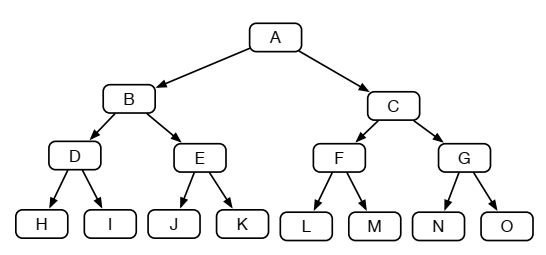
\includegraphics[scale=0.35]{images/lec06-pic01.png}
	\end{figure}
	\begin{block}{Полное бинарное дерево}
		$T_H$ высоты $H$ есть бинарное дерево, у которого к корню прикреплены левое и правое полные бинарные поддеревья $T_{H-1}$ высоты $H-1$. 
	\end{block}
	Число узлов в дереве $T_H$ есть $N = 2^{H+1}-1$, $H=log_2(N+1)$.
\end{frame}
  
\begin{frame}[t]
	\begin{block}{Приоритетная очередь (priority queue)}
		очередь, элементы которой имеют приоритет, влияющий на порядок извлечения: первым извлекается наиболее приоритетный элемент.
	\end{block}
	\begin{figure}[h]
		\centering
		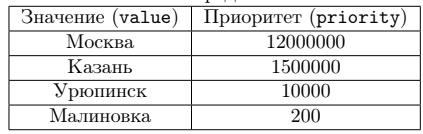
\includegraphics[scale=0.5]{images/lec06-pic02.png}
	\end{figure}	
	Интерфейс адстракции приоритетной очереди:
	\begin{itemize}
		\item insert -- добавляет элемент в очередь;
		\item fetchPriorityElement -- получает самый приоритетный элемент, но не извлекает его из очереди;
		\item extractPriorityElement -- извлекает самый приоритетный элемент из очереди.
	\end{itemize}
\end{frame}

\begin{frame}
	Использование упорядоченного массива:
	\begin{itemize}
		\item получение самого приоритетного элемента: отсортировать данные, взять последний элемент;
		\item извлечение элемента: $O(1)$;
		\item вставка элемента: поиск места вставки $O(log(N))$, сдвиг элементов вправо $O(N)$.
	\end{itemize}
\end{frame}

\begin{frame}
	\begin{block}{Бинарная куча (пирамида, heap)}
		 бинарное дерево, удовлетворяющее следующим условиям:
		 \begin{enumerate}
			\item Приоритет любой вершины не меньше приоритета потомков.
			\item Дерево является правильным подмножеством полного бинарного, допускающим плотное хранение узлов в массиве.		 
		 \end{enumerate}
	\end{block}
	В невозрастающей пирамиде приоритет каждого родителя не меньше приоритета потомков.
	\begin{figure}[h]
		\centering
		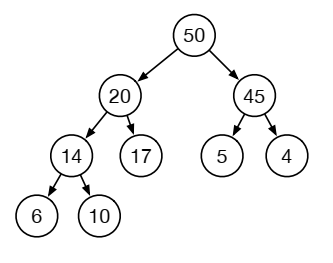
\includegraphics[scale=0.5]{images/lec06-pic03.png}
	\end{figure}		
\end{frame}

\begin{frame}
	Бинарная куча:
	\begin{figure}[h]
		\centering
		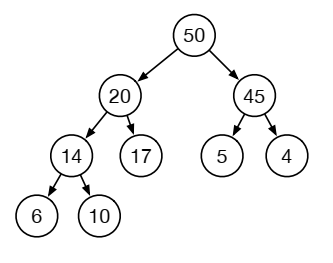
\includegraphics[scale=0.5]{images/lec06-pic03.png}
	\end{figure}		
	Хранение бинарной кучи в виде массива с индексами 1..N:
	\begin{figure}[h]
		\centering
		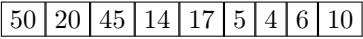
\includegraphics[scale=0.5]{images/lec06-pic04.png}
	\end{figure}
	Удобство такого хранения трудно переоценить:
	\begin{itemize}
		\item Индекс корня всегда равен $1$ -- самый приоритетный элемент.
		\item Индекс родителя узла $i$ всегда равен $\lfloor \frac{i}{2}\rfloor$.
		\item Индекс левого потомка узла $i$ всегда равен $2i$:
		\item Индекс правого потомка узле $i$ всегда равен $2i+1$:
	\end{itemize}
\end{frame}

\begin{frame}[fragile, t]
	Структура узла бинарной кучи:
	\begin{minted}{c}
struct bhnode { // Узел
	string data;
	int priority;
};	
	\end{minted}
	
	Бинарная куча:
	\begin{minted}{c}
struct binary_heap { 
	bhnode *body;
	int bodysize;
	//Будем фиксировать количество помещённых в кучу элементов в переменной numnodes. 	
	int numnodes;
	binary_heap(int maxsize);
	...
};	
	\end{minted}
\end{frame}

\begin{frame}[fragile, t]
	\begin{minted}{c}
//Операция создания бинарной кучи определённого размера заключается в простом выделении памяти под массив, хранящий элементы. 
//Нулевой элемент массива мы использовать не будем.	
binary_heap::binary_heap(int maxsize) {
	body = new bhnode[maxsize+1];
	bodysize = maxsize;
	numnodes = 0;
}
~binary_heap::binary_heap() {
	delete body;
}
//Ещё нам понадобится операция обмена элементов кучи по их индексам:
void binary_heap::swap(int a, int b) {
	std::swap(body[a],body[b]);
}
	\end{minted}
\end{frame}

\begin{frame}[fragile]
	Сложность операции создания бинарной кучи -- $T_{create}=O(N)$.
	
	~
	
	Операция поиска самого приоритетного элемента тривиальна. Её сложность -- $T_{fetchMin}=O(1)$:
	\begin{minted}{c}
bhnode *binary_heap::fetchPriorityElement() {
	return numnodes == 0? nullptr : body + 1;
}
	\end{minted}
	
	~
	
	Правильная бинарная куча должна поддерживать два инварианта:
	\begin{itemize}
		\item структурную целостность: представимости в виде бинарного дерева
		\item упорядоченную целостности: то есть свойства <<потомки узла не могут иметь приоритет, больший, чем у родителя>>. 
	\end{itemize}	
\end{frame}

\begin{frame}{Добавление элемента в бинарную кучу}
	\textbf{Этап 1}: вставка в конец кучи
	\begin{figure}[h]
		\centering
		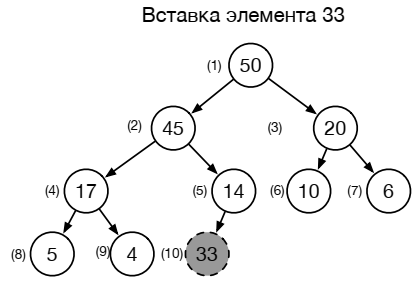
\includegraphics[scale=0.5]{images/lec06-pic05.png}
	\end{figure}
	Отлично! Структура кучи не испортилась!
	\begin{figure}[h]
		\centering
		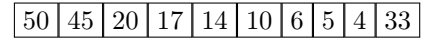
\includegraphics[scale=0.5]{images/lec06-pic06.png}
	\end{figure}	
	Однако пока не выдержана упорядоченность.
\end{frame}

\begin{frame}{Добавление элемента в бинарную кучу}
	\textbf{Этап 2}: Корректировка значений
	
	~
	
	Только что вставленный элемент может оказаться более приоритетным, чем его родитель. Тогда поменяем их местами.
	\begin{figure}[h]
		\centering
		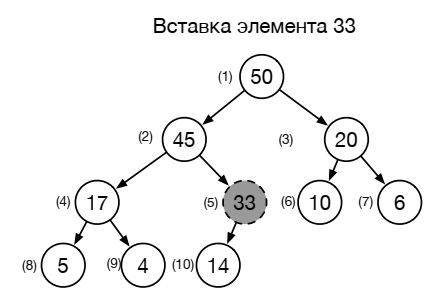
\includegraphics[scale=0.5]{images/lec06-pic07.png}
	\end{figure}
	Куча удовлетворяет всем условиям.
	\begin{figure}[h]
		\centering
		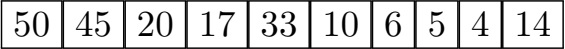
\includegraphics[scale=0.4]{images/lec06-pic08.png}
	\end{figure}	
\end{frame}

\begin{frame}{Добавление элемента в бинарную кучу}	
	Попытаемся вставить элемент, который имеет приоритет больше, чем все элементы в куче.
	\begin{figure}[h]
		\centering
		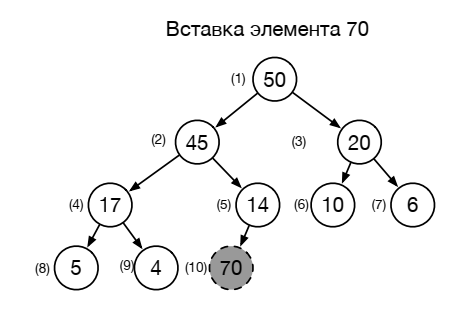
\includegraphics[scale=0.4]{images/lec06-pic09.png}
	\end{figure}
	Он находится не на своём месте... 
	\begin{figure}[h]
		\centering
		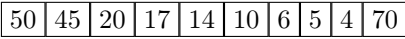
\includegraphics[scale=0.5]{images/lec06-pic10.png}
	\end{figure}	
\end{frame}

\begin{frame}{Добавление элемента в бинарную кучу}	
	... и меняется местами с родителем (ползёт вверх по дереву).
	\begin{figure}[h]
		\centering
		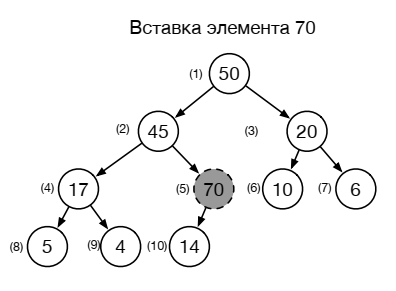
\includegraphics[scale=0.4]{images/lec06-pic11.png}
	\end{figure}
	Опять он не на своём месте — и опять меняется местами с родителем.
	\begin{figure}[h]
		\centering
		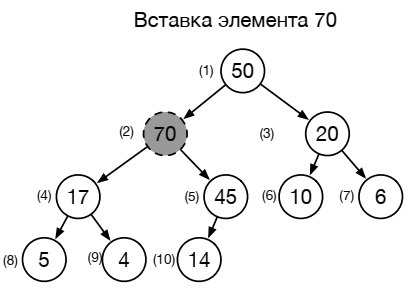
\includegraphics[scale=0.4]{images/lec06-pic12.png}
	\end{figure}
\end{frame}

\begin{frame}{Добавление элемента в бинарную кучу}	
	Максимальный элемент переместился в корень. 
	\begin{figure}[h]
		\centering
		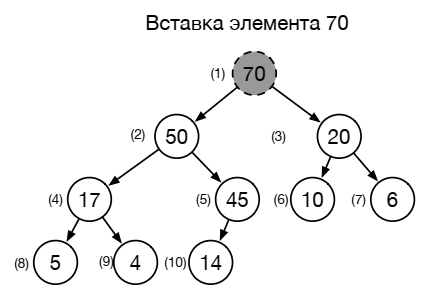
\includegraphics[scale=0.4]{images/lec06-pic13.png}
	\end{figure}
	Алгоритм завершён
	\begin{figure}[h]
		\centering
		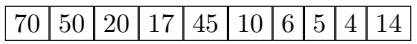
\includegraphics[scale=0.4]{images/lec06-pic14.png}
	\end{figure}	
\end{frame}

\begin{frame}[fragile]
	Корректность алгоритма базируется на двух фактах:
	\begin{itemize}
		\item Инвариант структурной целостности не нарушен ни в один момент времени.
		\item После каждого шага перемещения вставленного элемента поддерево с корнем в текущем элементе поддерживает инвариант упорядоченной
целостности.
	\end{itemize}
	Сложность алгоритма определяется высотой дерева и составляет $T_{Insert}=O(log(N))$.
	\begin{minted}{c}
int binary_heap::insert(bhnode node) {
	if (numnodes > bodysize) {
		return -1; // или расширяем.
	}
	body[++numnodes] = node;
	for (int i = numnodes; i > 1 && 
		body[i].priority > body[i/2].priority; i /= 2) {
		swap(i, i/2);
	}
}	
	\end{minted}
\end{frame}

\begin{frame}{Операция удаления самого приоритетного элемента}
	\begin{itemize}
		\item Операция удаления самого приоритетного элемента кажется более сложной -- ведь после удаления корневого элемента нарушается структурная целостность. 
		\item Первый шаг при удалении корневого элемента должен сохранять структурную целостность. 
		\item Так как после удаления корня количество элементов уменьшится на один, то отправляем самый последний элемент кучи в корень, уменьшая при этом numnodes.	
	\end{itemize}
	\begin{figure}[h]
		\centering
		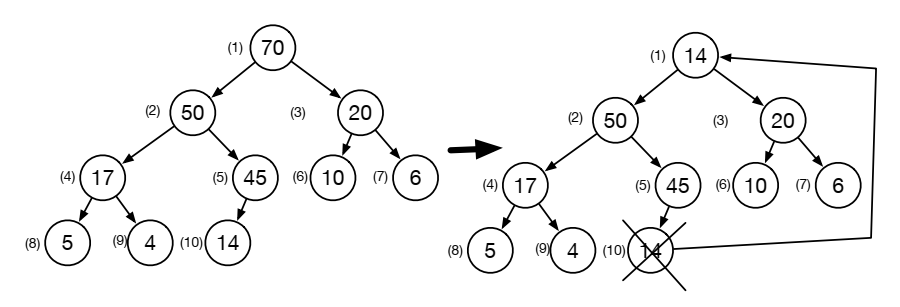
\includegraphics[scale=0.5]{images/lec06-pic15.png}
	\end{figure}	
\end{frame}

\begin{frame}{Операция удаления самого приоритетного элемента}
	\begin{itemize}
		\item Операция удаления самого приоритетного элемента кажется более сложной -- ведь после удаления корневого элемента нарушается структурная целостность. 
		\item Первый шаг при удалении корневого элемента должен сохранять структурную целостность. 
		\item Так как после удаления корня количество элементов уменьшится на один, то отправляем самый последний элемент кучи в корень, уменьшая при этом numnodes.	
	\end{itemize}
	\begin{figure}[h]
		\centering
		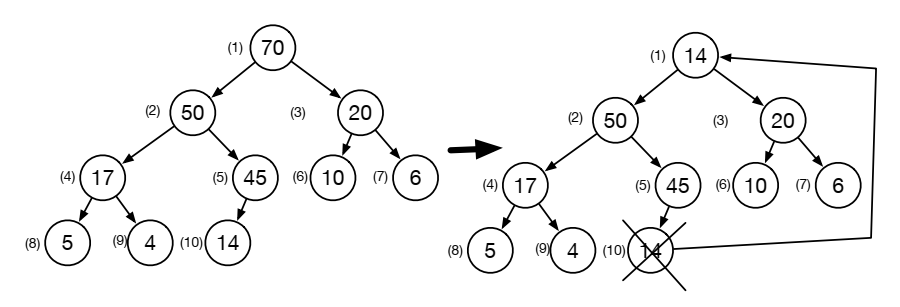
\includegraphics[scale=0.5]{images/lec06-pic15.png}
	\end{figure}	
\end{frame}

\begin{frame}
	Структурная целостность не изменилась, но могла измениться упорядоченная целостность. Требуется восстановление, функция heapify.
	\begin{itemize}
		\item Идея функции проста: начиная с корневого элемента, мы проводим соревнование между тремя кандидатами -- теми, кто может занять это место.
		\item Если кандидаты (левый и правый потомки) менее приоритетны, чем текущий претендент, то алгоритм завершён. 
		\item Иначе претендент меняется местами с самым приоритетным из потомков -- и операция повторяется уже на
уровне ниже. Так как каждая операция обмена передвигает претендента на один уровень вниз, процесс обязательно завершается не более, чем за $O(log N)$ шагов, что и составляет сложность данного алгоритма.	
	\end{itemize}
\end{frame}

\begin{frame}	
	Проиллюстрируем алгоритм на примере. 
	\begin{itemize}
		\item После перемещения последнего узла (14) в корень он становится претендентом, а кандидатами оказываются узлы (50) и (20). 
		\item Индекс восстановления (номер претендента) пока равен 1.
	\end{itemize}
	\begin{figure}[h]
		\centering
		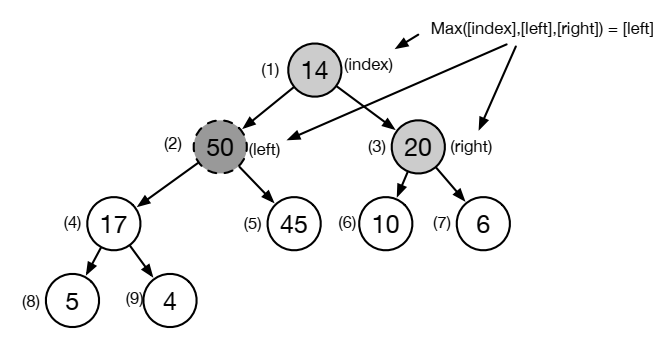
\includegraphics[scale=0.5]{images/lec06-pic16.png}
	\end{figure}	
\end{frame}

\begin{frame}
	\begin{itemize}
		\item Претендента обменяли на кандидата (50) с индексом 2. 
		\item Теперь элемент под этим индексом -- новый претендент.
	\end{itemize}
	\begin{figure}[h]
		\centering
		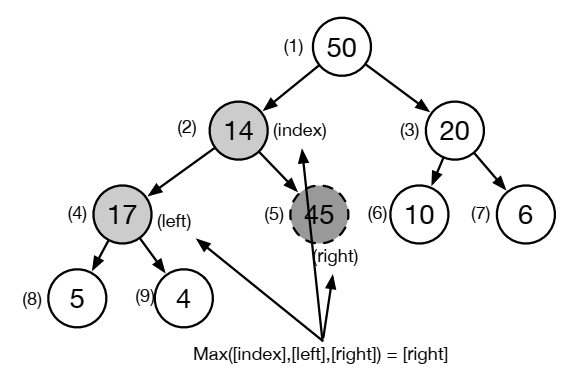
\includegraphics[scale=0.5]{images/lec06-pic17.png}
	\end{figure}	
\end{frame}

\begin{frame}
	\begin{itemize}
		\item Теперь претендентом становится элемент с индексом 5. 
		\item После завершения этой операции восстановление завершено.
	\end{itemize}
	\begin{figure}[h]
		\centering
		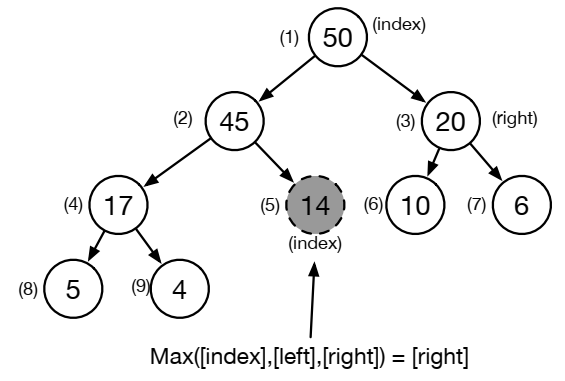
\includegraphics[scale=0.5]{images/lec06-pic18.png}
	\end{figure}	
\end{frame}

\begin{frame}[fragile]
	\begin{minted}{c}
void binary_heap::heapify(int index) {
  for (;;) {
    int left = index + index;
    int right = left + 1;
    // Кто больше, [index], [left], [right]?
    int largest = index;
    if (left <= numnodes &&
        body[left].priority > body[index].priority)
      largest = left;
    if (right <= numnodes &&
        body[right].priority > body[largest].priority)
      largest = right;
    if (largest == index) break;
    swap(index, largest);
    index = largest;
  }
}
	\end{minted}
\end{frame}

\begin{frame}{Алгоритм HeapSort}
	Возможность получать из бинарной кучи самый приоритетный элемент за $O(log N)$ и добавлять элементы в бинарную кучу за $O(log N)$ вызывает желание реализовать ещё один алгоритм сортировки. Что интересно, этот
алгоритм будет иметь сложность $O(N log N)$ в худшем случае.
	\begin{enumerate}
		\item Создать бинарную кучу размером $N$. Это потребует сложности $O(N)$.
		\item Поочерёдно вставить в неё все $N$ элементов массива. Сложность этого этапа есть
$O(log 1)+O(log 2)+...+O(log N))<O(log N)+...+O(log N))=N log(N)$.
		\item Поочерёдно извлекать с удалением самый приоритетный элемент из бинарной кучи - -с помещением в последовательные $N$ позиций исходного массива.
	\end{enumerate}
	Такая прямолинейная организация не особенно хороша: потребуется добавочная память на бинарную кучу размером N элементов.
\end{frame}

\begin{frame}[fragile]
	Модифицируем функцию heapify для того, чтобы она могла работать с произвольным массивом, адресуемым с нуля:
	\begin{minted}{c}
void heapify(int *a, int i, int n){
  int curr = a[i];
  int index = i;
  for (;;) {
    int left = index + index + 1;
    int right = left + 1;
    if ( left < n && a[left] > curr)
      index = left;
    if ( right < n && a[right] > a[index])
      index = right;
    if (index == i ) break;
    a[i] = a[index];
    a[index] = curr;
    i = index;
  }
}
	\end{minted}
\end{frame}

\begin{frame}[fragile]{Алгоритм HeapSort}
	\begin{itemize}
		\item Теперь сортировка заключается в том, что мы создаём бинарную кучу размером $n$ на месте исходного массива, переставляя его элементы. 
		\item Затем на шаге $i$ мы обмениваем самый приоритетный элемент кучи (он всегда располагается на позиции $0$) с элементом под номером $n-i-1$. 
		\item Размер кучи при этом уменьшается на единицу, а самый приоритетный элемент занимает теперь положенное ему по рангу место.
	\end{itemize}
\end{frame}

\begin{frame}[fragile]
	\begin{minted}{c}
void sort_heap(int *a, int n) {
  for(int i = n/2-1; i >= 0; i--) {
    heapify(a, i, n);
  }
  while( n > 1 ) {
    n--;
    swap(a[0],a[n]);
    heapify(a, 0, n);
  }
}
	\end{minted}
	
	Вопрос: если эта сортировка гарантирует нам сложность $O(N log(N))$ даже в самом худшем случае, а быстрая сортировка, QuickSort, не гарантирует, то почему не использовать только эту сортировку? 
\end{frame}

\begin{frame}[fragile]{Алгоритм HeapSort}
	\begin{enumerate}
		\item Первая причина в том, что в быстрой сортировке используется меньшее количество операций обмена с памятью, а излишней работы с памятью на современных компьютерах стоит избегать. 
		\item Вторая причина тоже связана с памятью, точнее -- с тем фактом, что N обращений к последовательным
ячейкам памяти исполняется до 10-15 раз быстрее, чем столько же обращений к случайным ячейкам памяти. Это связано с наличием ограниченного количества аппаратной кэш-памяти на современных процессорах. 
	\end{enumerate}
	При наличии различных алгоритмов, исполняющих одну и ту же задачу, некоторые из них могут быть дружелюбны к кэшу (cache-friendly), а некоторые -- нет. Поэтому наилучшие по времени исполнения алгоритмы могут быть разными в различное время и на различных вычислительных системах.	
\end{frame}

\end{document}
